%% NOVAC
%% =============
%%

\begin{figure}[h]
	\centering
	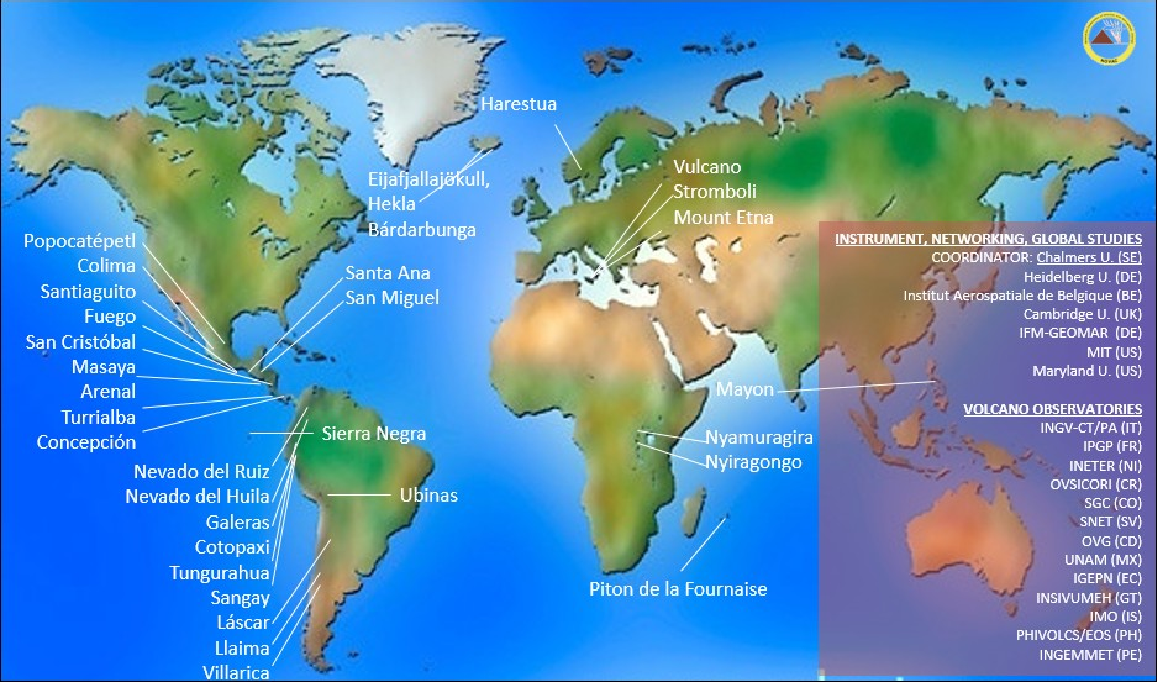
\includegraphics[width=0.8\linewidth]{Bilder/NOVAC2015}
	\caption{Global map of the volcanoes monitored by NOVAC. Used with friendly permission of Santiago Arellano.}
	\label{fig:novac2015}
\end{figure}
The Network for Observation of Volcanic and Atmospheric Change (NOVAC) is a network of instruments monitoring volcanoes over the whole world. 
%
NOVAC was installed to add a monitoring parameter for volcanic activity by installing automatized instruments measuring \ce{SO2} emissions during the daytime.\\
%
NOVAC was originally a European funded research project from 2005 until 2010. The aim of NOVAC is to establish a global network of stations for the quantitative measurement of volcanic gas emissions in particular \ce{SO2}. At the beginning, NOVAC encompassed observatories of 15 volcanoes in Africa, America and Europe, including some of the most active and strongest degassing volcanoes in the world. Although the EU-funding has stopped, the network has been constantly growing since it was founded. In 2018 more than 100 instruments are installed at over 40 volcanoes in more than 13 countries.
\Cref{fig:novac2015} shows a map, with all volcanoes of the Network for Observation of Volcanic and Atmospheric Change.\\

The great advantage of the data monitored in NOVAC is the fact that NOVAC provides continues gas emission data over many years. This ensures statistically meaningful results for the data evaluation.\\
The instruments used in NOVAC are scanning UV-spectrometer named Mini DOAS instruments. \\
The  Mini DOAS instrument represents a major breakthrough in volcanic gas monitoring as it is capable of real-time semi-continuous unattended measurement of the total emission fluxes of  \ce{SO2} and BrO from a volcano. In this case, semi-continues means that the measurement is only possible during the daytime.\\
%
\begin{figure}
	\centering
	%    \subfigure[ ]
	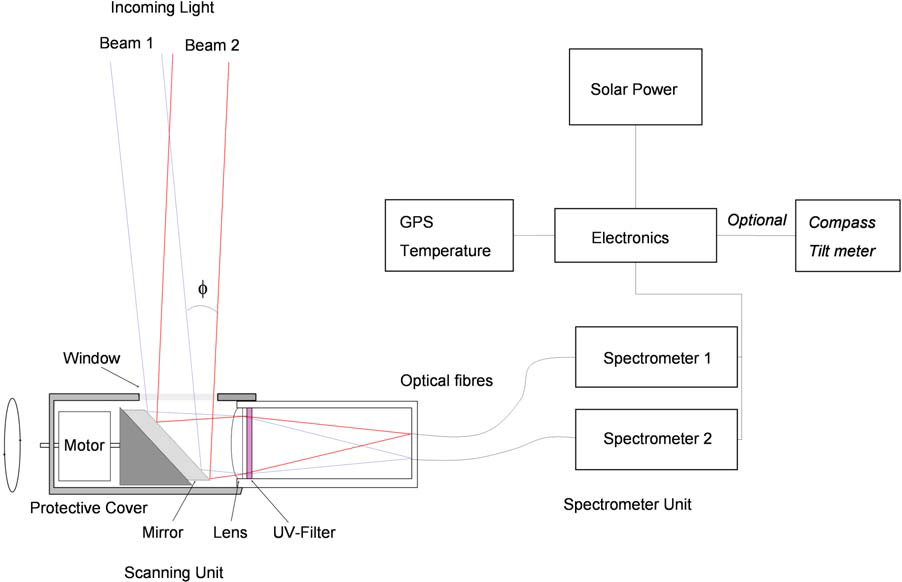
\includegraphics[width=1\textwidth]{Bilder/Simon/Bilder_Tung/NOVAC_Instrument}
	%    \subfigure[Different Scan geometrys of NOVAC-Instruments From \cite{galle2010network}]{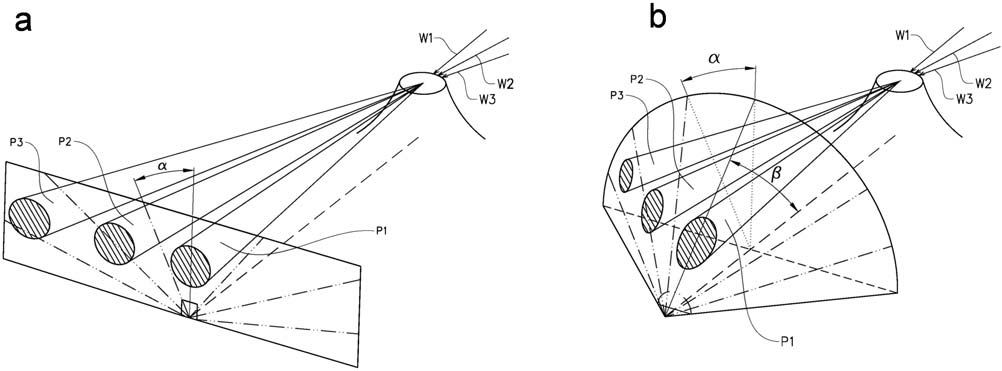
\includegraphics[width=0.49\textwidth]{Bilder/Simon/Bilder_Tung/NOVAC_scan_geo}}
	\caption{schematic sketch of a NOVAC instrument. From \cite{galle2010network}}
\end{figure}
The  basic  Mini DOAS  system  consists  of  a  pointing  telescope  fiber-coupled  to  a  spectrograph.  
Ultraviolet light from the sun, scattered from aerosols and molecules in the atmosphere, is collected by 
means  of  a  telescope  with  a  quartz  lens  defining  a  field-of-view  of  12~mrad
\citep{NOVACsite}. \\
The spectrometers measure in the UV region in a wavelength range of 280 to 420~nm. In this range the differential structures of \ce{SO2} and BrO structures are dominant.\\
The lack of temperature stabilization at the instruments used by NOVAC comes with a reduced precision of the data, but the huge amount of data produced by NOVAC compensates for this limitation.  
%        \textcolor{red}{naja und es kommt evben auch immer drauf an was fuer genauigkeiten man bracuht - wenn ich eine groessenordnung in der emissionsmessungen sehen will muss ich nicht auf ein promille genau messen,..}


\section{Measurement routine}
\begin{figure}[h]
	\hspace*{-0.8cm}
	\subfigure{
		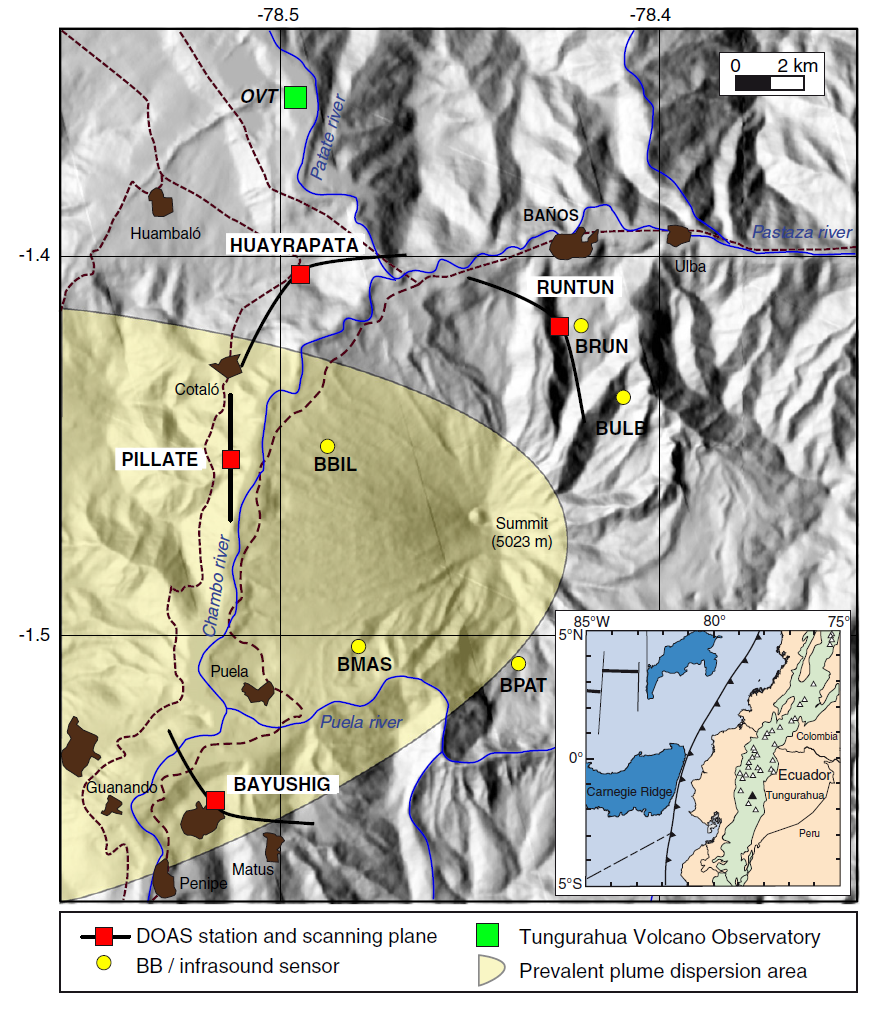
\includegraphics[width=0.488\linewidth]{Bilder/Simon/Bilder_Tung/Map_Tungurahua2}}
	\subfigure{
		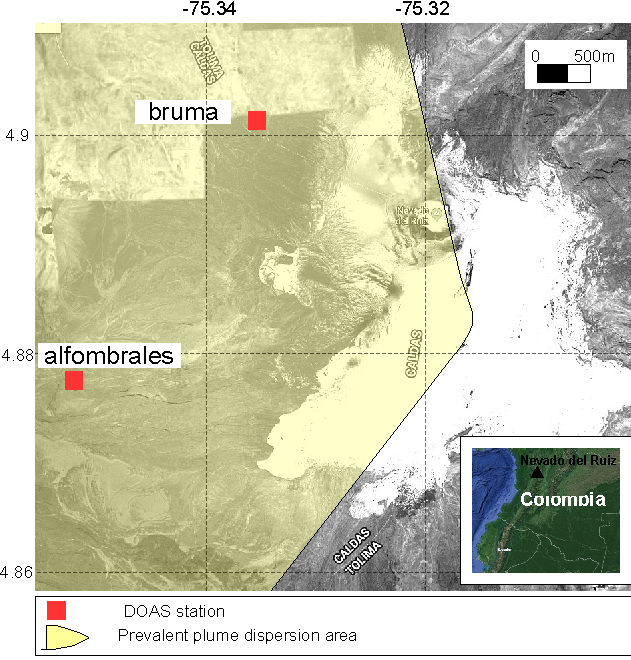
\includegraphics[width=0.542\linewidth]{Bilder/NdR_map}}
	\caption[Topographig Map of the Tungurahua Volcano ( from \cite{hidalgo2015so2}) and Nevado del Ruiz volcano]{Topographig Map of the Tungurahua Volcano (left, from \cite{hidalgo2015so2}) and Nevado del Ruiz volcano (right). The predominant plume direction is shaded in yellow.  The NOVAC stations are shown as red squares, the corresponding scanning geometry is sketched with black lines. The prevalent plume dispersion is taken from the wind rose shown in \citet{Windrose} the topographic map is taken from google maps.}
	\label{fig:maptungurahua2}
\end{figure}

The instruments are set up five to ten km downwind of the volcano. To cover most of the occurring wind directions two to five instruments are installed at each volcano. Ideally, the measurement plane is orthogonal to the plume, to get the best measurement results. In reality, the measurement plane might be rotated.\\

For the calculations of gas data from the DOAS retrieval, a spectrum of the plume (plume spectrum) and a scan without any volcanic trace gases (reference spectrum) is needed.  This is done without any knowledge of the plume location by scanning the whole sky. 
The measurement routine starts with a spectrum in zenith direction: the pre-reference. The exposure time of the pre-reference will be used for the whole scan.
Afterward, the dark current spectrum is recorded for the correction of the dark and offset.\\
Then the telescope turns automatically to the side, recording spectra at the elevation angle from -90$^{\circ}$ to 90$^{\circ}$ with steps of 3.6$^{\circ}$. \\
The instruments record 53 spectra per scan, the pre-reference, the dark current spectrum and 51 spectra at different elevation angles.
One whole measurement cycle from horizon to horizon takes 6 to 15 minutes depending on the current illumination conditions.


\subsection*{Tungurahua \label{Tung}}
\begin{table}
	\centering
	\begin{tabular}{|p{4cm}|p{3cm}|p{3cm}|p{3cm}|}
		%    \toprule
		Instrument    &D2J2140&I2J8546& I2J8548\\
		\toprule
		compass&90.0    &    30.0    &    360.0    \\
		latitude&-1.453584    &    -1.543492    &-1.404719    \\
		longitude&-78.513047    &-78.517179    &    -78.494777    \\
		altitude&2609.980    &    2782.352    &    2911.253    \\
		volcano&Tungurahua    &Tungurahua    &    Tungurahua    \\
		site&pillate    &    bayushig    &    huayrapata    \\
		observatory&igepn    &    igepn    &igepn    \\
		serial&D2J2140    &    I2J8546    &    I2J8548    \\
		spectrometer&S2000    &    S2000    &S2000    \\
		instrumenttype&gothenburg    &gothenburg    &gothenburg    \\
		version&2.1    &2.1    &    2.1    \\
		\bottomrule
	\end{tabular}
	\caption{Technical data of the instruments installed at the Tungurahua volcano.}
	\label{tab:TInstruments}
\end{table}
Tungurahua is a steep-sided andesitic-dacitic subduction zone volcano located in the Ecuadorian Andes (Lat: 1.467$^{\circ}$S; Long: 78.442$^{\circ}$W). 2014 Tungurahua was one of the most active volcanoes in southern America since then, the activity is decreasing. Tungurahua is 5023m high and is one of the defining volcanoes of the eastern volcanic rows in Ecuador \citep{hall1999tungurahua}.
\\
The modern volcano was formed by a sequential construction of three major edifices on a basement of metamorphic rocks. It has a total diameter of 12 km. Tungurahua I was roughly located at the same place as today and was build up in the mid-Pleistocene, mainly by andesitic and dacitic lava flows as well as interbedded tephra. Tungurahua II was formed in the past 14,000 years as a result of the collapse of the initial edifice.\\
3000 years ago the Tungurahua II edifice collapse. The collapse of Tungurahua II produced a large debris-avalanche deposit and a horseshoe-shaped caldera which is open to the west side. Tungurahua III the current glacier caped stratovolcano was constructed in this caldera \citep{GlobalVolcanismProgram}.\\
The current ongoing long-term eruption started in October 1999. The eruptive phase was preceded by hydrothermal tremors between 1994 and 1997 \citep{samaniego2003peligros}.\\
From September 1998 to July 1999 an increase of seismic activity like volcano-tectonic earthquakes indicated the raising of magma. This eruptive phase was characterized by alternating periods of high and low volcanic activity. \\

At Tungurahua, three instruments described in \cref{tab:TInstruments}, with data recorded in the time span from July in 2008 to August in 2009, are used in this thesis.
\Cref{tab:TInstruments} shows the exact position, of the instruments, the altitude, and other specifications. \\

\subsection*{Nevado del Ruiz}
Nevado del Ruiz is a glacier-covered, subduction zone volcano which is located in the Central Cordillera of Colombia, 140 km west of Bogota
(Lat: 4.892$^{\circ}$N; Long: 75.324$^{\circ}$W). Nevado De Ruiz has a hight of 5389 m and covers an area of more than 200 km$^2$.
Three major edifices have been constructed since the beginning of the Pleistocene, consisting of andesitic and dacitic lavas and pyrolastics \citep{GlobalVolcanismProgram}. \\
The current cone is built within the caldera of the older edifice and consists of a cluster of lava domes. The crater on the summit, with the name Arenas crater, has a diameter of 1 km and a depth of 240 m. 
The last big eruption was in 1985. This was South America's deadliest eruption.\\
In this thesis, the data of two NOVAC instruments (see \cref{tab:NVDRInstruments}) in the time from the end of 2009 to the end of 2011 are used. \\
\\
\begin{table}
	\centering
	\begin{tabular}{|p{4cm}|p{3cm}|p{3cm}|}
		%    \toprule
		Instrument    &D2J2200&D2J2201\\
		\toprule
		compass&115.0        &59.0        \\
		tilt&0.0        &0.0        \\
		latitude&4.900917        &4.876183        \\
		longitude&-75.335134        &-75.353408        \\
		altitude&4866.500        &4494.259        \\
		volcano&Nevado del Ruiz        &Nevado del Ruiz        \\
		site&bruma    &alfombrales\\
		observatory&ingeominas        &ingeominas        \\
		serial&D2J2200        &D2J2201        \\
		spectrometer&S2000        &S2000        \\    
		instrumenttype &gothenburg        &gothenburg        \\
		version&2.2        &2.2        \\
		softwareversion &1.82        &1.82        \\
		compiledate &Feb 19 2009        &Feb 19 2009        \\
		\bottomrule
	\end{tabular}
	\caption{Technical data of the instruments installed at the Nevado del Ruiz volcano.}
	\label{tab:NVDRInstruments}
\end{table}